\begin{frame}
    \frametitle{Uživatelská dokumentace}

    \begin{block}{Uživatelská dokumentace}
        \textbf{Uživatelská dokumentace} je důležitá pro uživatele knihovny, kteří se snaží pochopit, jak knihovnu používat.
        Měla by být jednoduchá a srozumitelná. Měla by zároveň popisovat jednotlivé funkce knihovny.
    \end{block}
\end{frame}

\begin{frame}
    \frametitle{Uživatelská dokumentace - TypeDoc}
    \framesubtitle{Generování dokumentace z kódu}

    \begin{block}{TypeDoc}
        TypeDoc je nástroj, který umožňuje generovat dokumentaci z kódu.
        Dokumentace je generována z komentářů v kódu.
    \end{block}
\end{frame}

\begin{frame}
    \frametitle{Uživatelská dokumentace - TypeDoc}
    \framesubtitle{Ukázka komentáře v JSDoc syntaxi}

    \begin{figure}
        \centering
        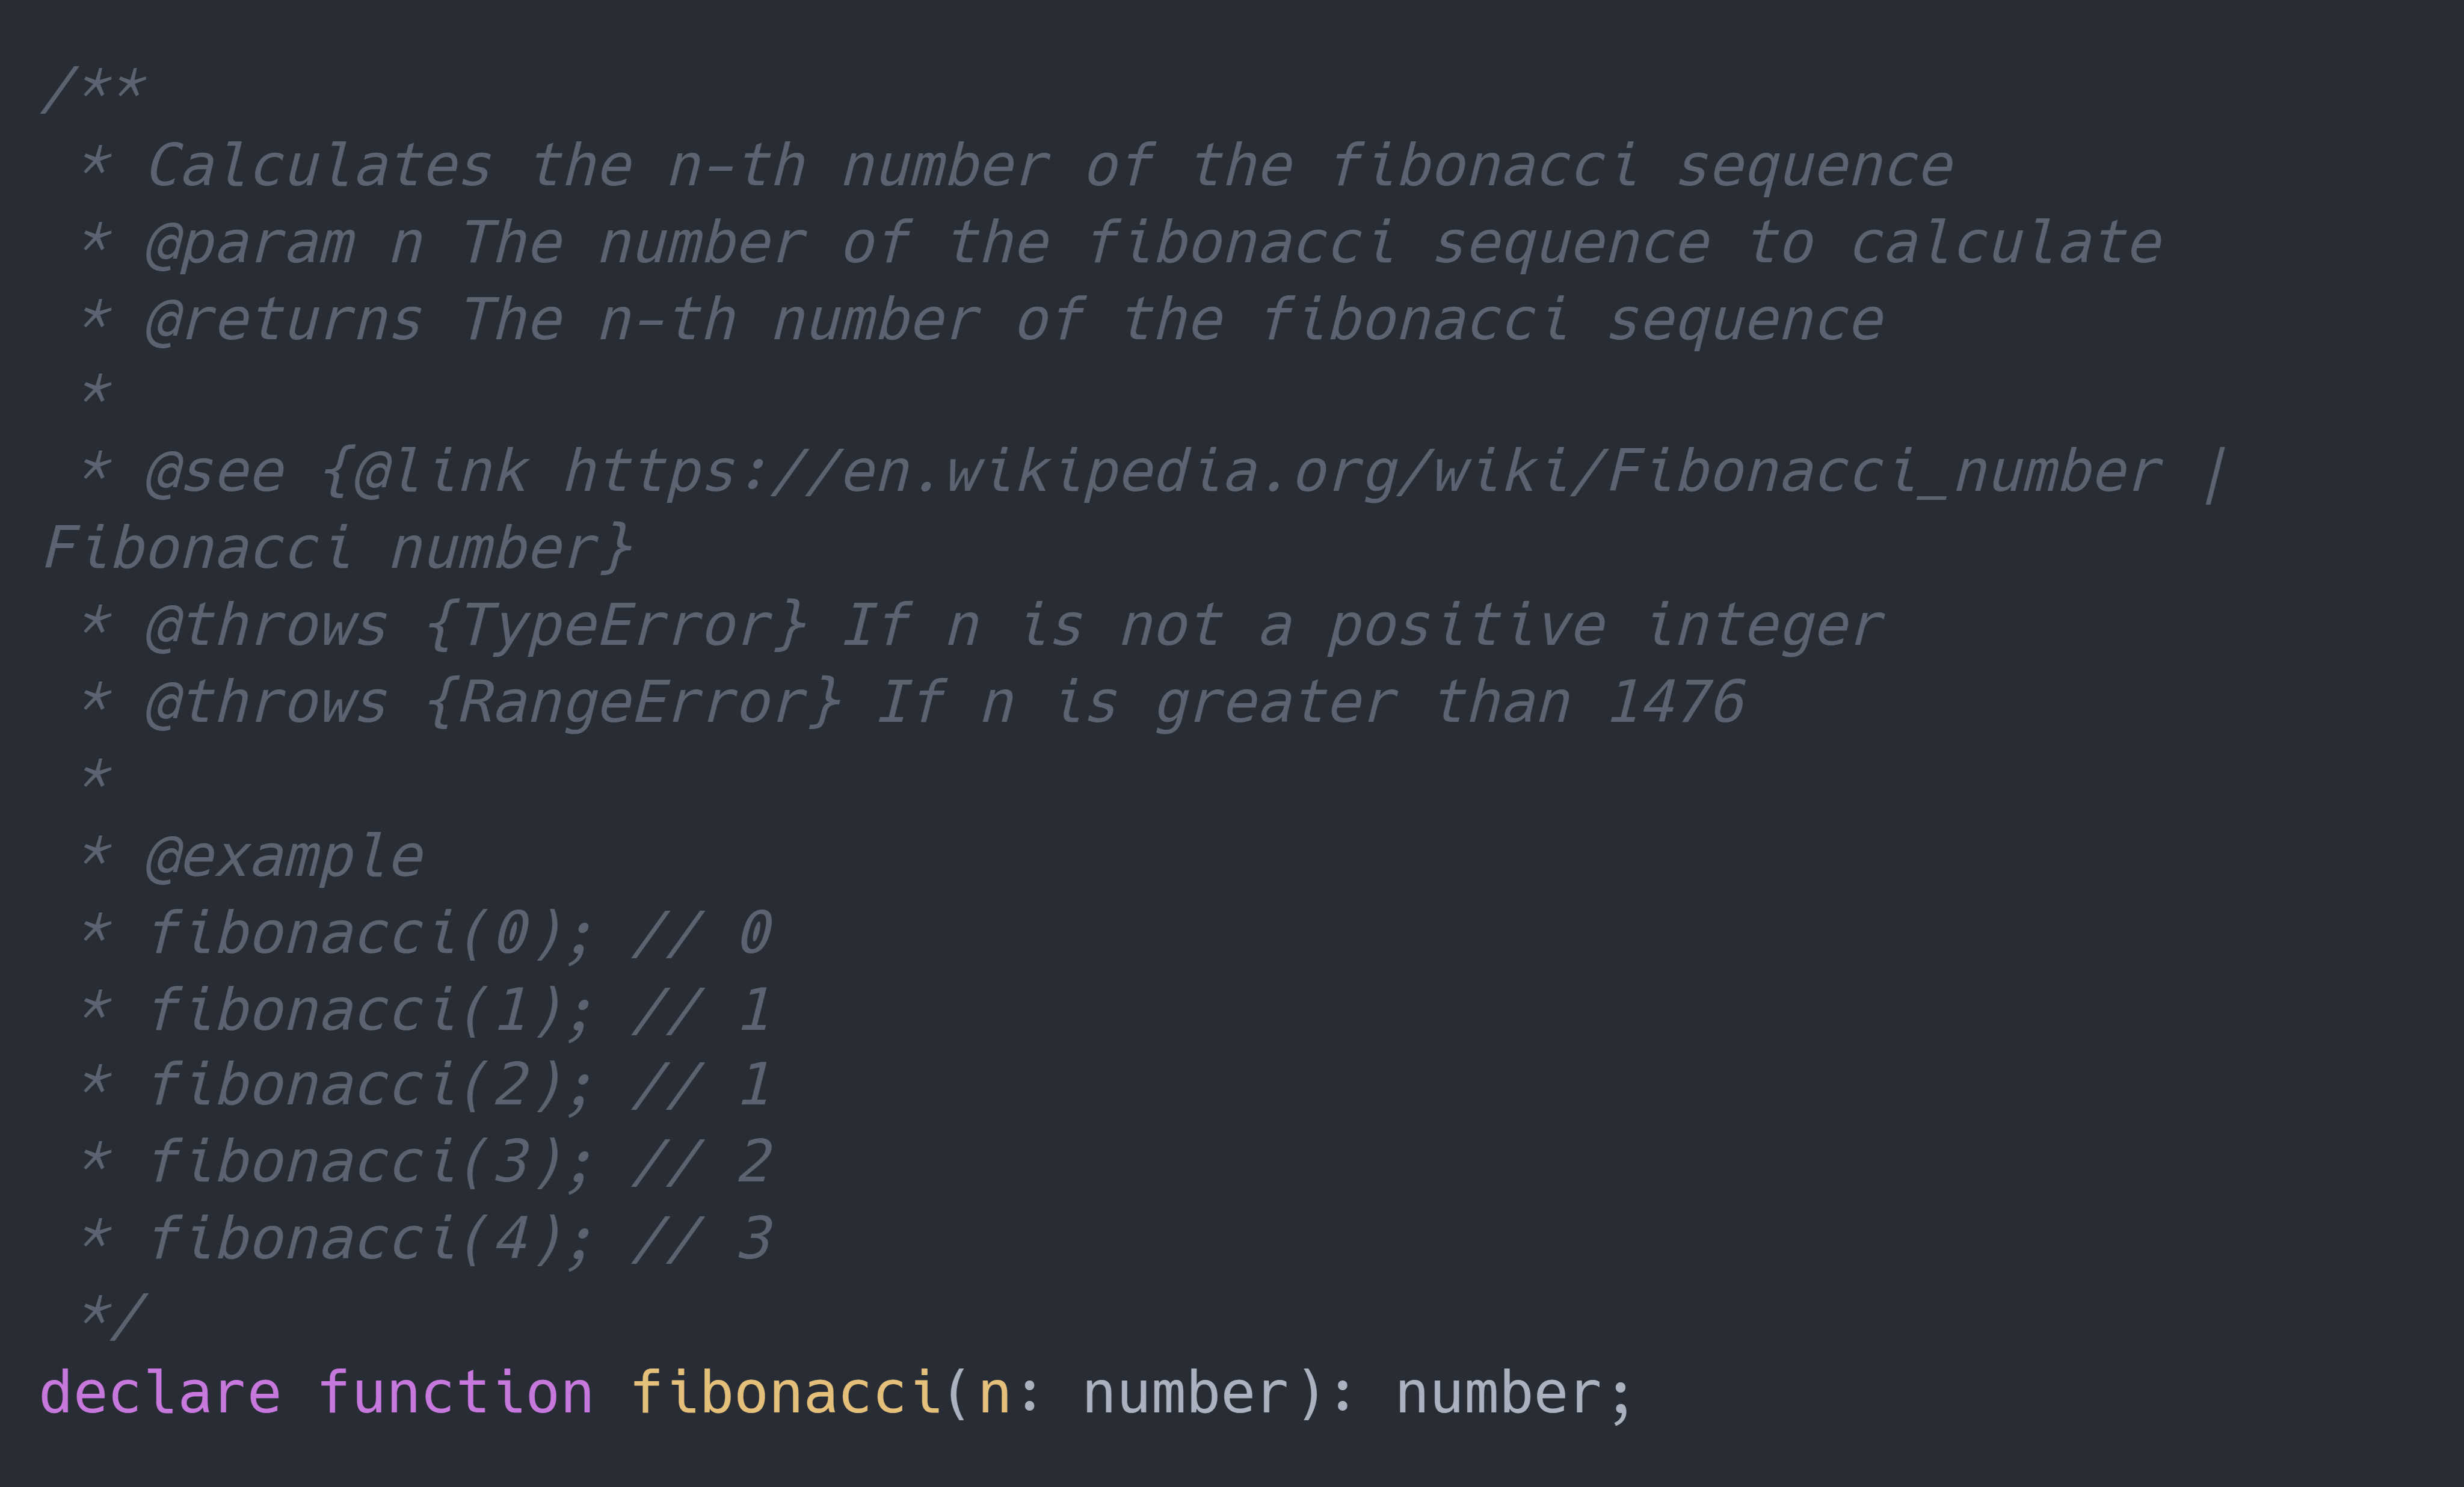
\includegraphics[height=0.65\textheight]{../resources/snippets/typeDoc/comment_example.ts.png}
        \caption{Ukázka komentáře v JSDoc syntaxi.}
    \end{figure}
\end{frame}

\begin{frame}
    \frametitle{Uživatelská dokumentace - TypeDoc}
    \framesubtitle{Ukázka metody \texttt{normalize} rozhraní \texttt{Vector}}
    \begin{figure}
        \centering
        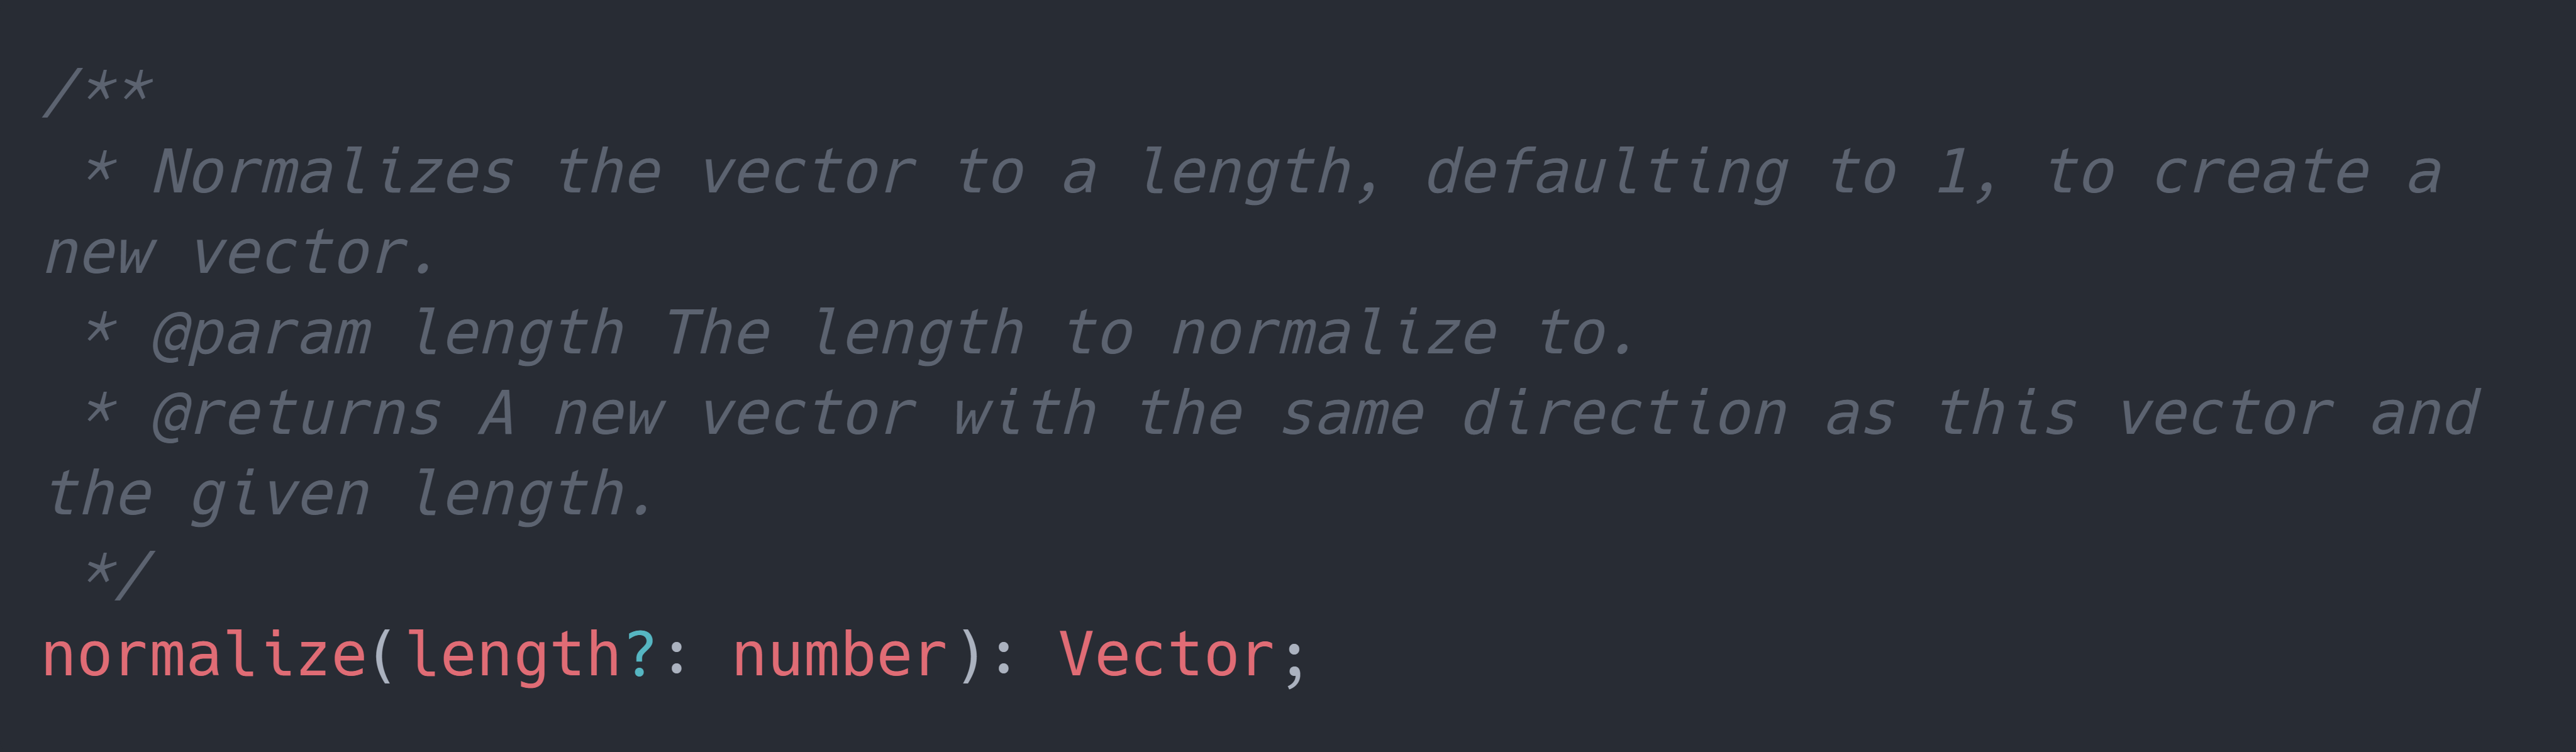
\includegraphics[height=0.5\textheight]{../resources/snippets/typeDoc/vector_normalize.ts.png}
        \caption{Ukázka komentáře v JSDoc syntaxi z knihovny.}
    \end{figure}
\end{frame}

\begin{frame}
    \frametitle{Uživatelská dokumentace - TypeDoc}
    \framesubtitle{Ukázka metody \texttt{normalize} rozhraní \texttt{Vector}}
    \begin{figure}
        \centering
        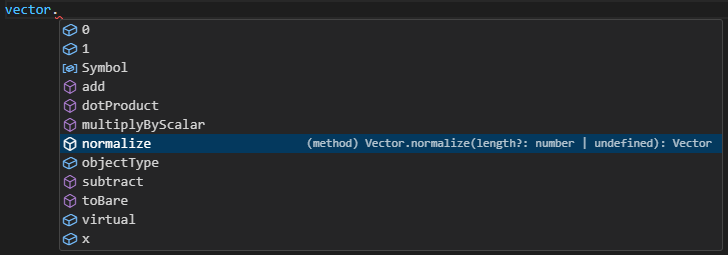
\includegraphics[height=0.6\textheight]{../resources/vector-normalize-suggestion-vscode.png}
        \caption{Ukázka IntelliSense v editoru Visual Studio Code.}
    \end{figure}
\end{frame}

\begin{frame}
    \frametitle{Uživatelská dokumentace - TypeDoc}
    \framesubtitle{Ukázka metody \texttt{normalize} rozhraní \texttt{Vector}}
    \begin{figure}
        \centering
        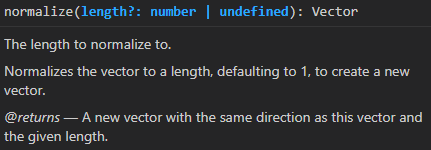
\includegraphics[height=0.5\textheight]{../resources/vector-normalize-documentation-vscode.png}
        \caption{Ukázka detailu IntelliSense v editoru Visual Studio Code.}
    \end{figure}
\end{frame}

\begin{frame}
    \frametitle{Uživatelská dokumentace - TypeDoc}
    \framesubtitle{Ukázka metody \texttt{normalize} rozhraní \texttt{Vector}}
    \begin{figure}
        \centering
        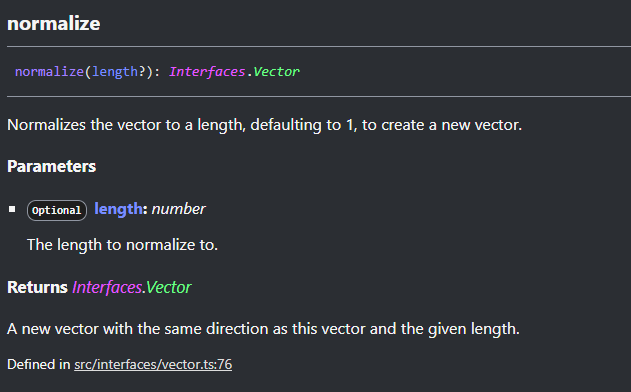
\includegraphics[height=0.65\textheight]{../resources/vector-normalize-documentation-typedoc.png}
        \caption{Ukázka webové dokumentace.}
    \end{figure}
\end{frame}


\begin{frame}
    \frametitle{Programátorská dokumentace}
    \framesubtitle{GitHub Wiki}
    \onslide<1->{
        \begin{block}{Programátorská dokumentace}
            \textbf{Programátorská dokumentace} je důležitá pro vývojáře, kteří chtějí přispívat do knihovny.
            Měla by obsahovat informace o tom, jak knihovnu spravovat, jak ji testovat a jak ji publikovat.
            Také by měla obsahovat informace o tom, jak knihovnu rozšířit.
        \end{block}
    }
    \onslide<2-> {
        \begin{block}{GitHub Wiki}
            GitHub Wiki je jednoduchý nástroj, který umožňuje vytvářet programátorskou dokumentaci.
            Je součástí každého repozitáře na GitHubu.
        \end{block}
    }
\end{frame}
\begin{frame}
    \frametitle{Programátorská dokumentace}
    \framesubtitle{GitHub Wiki}
    \begin{figure}
        \centering
        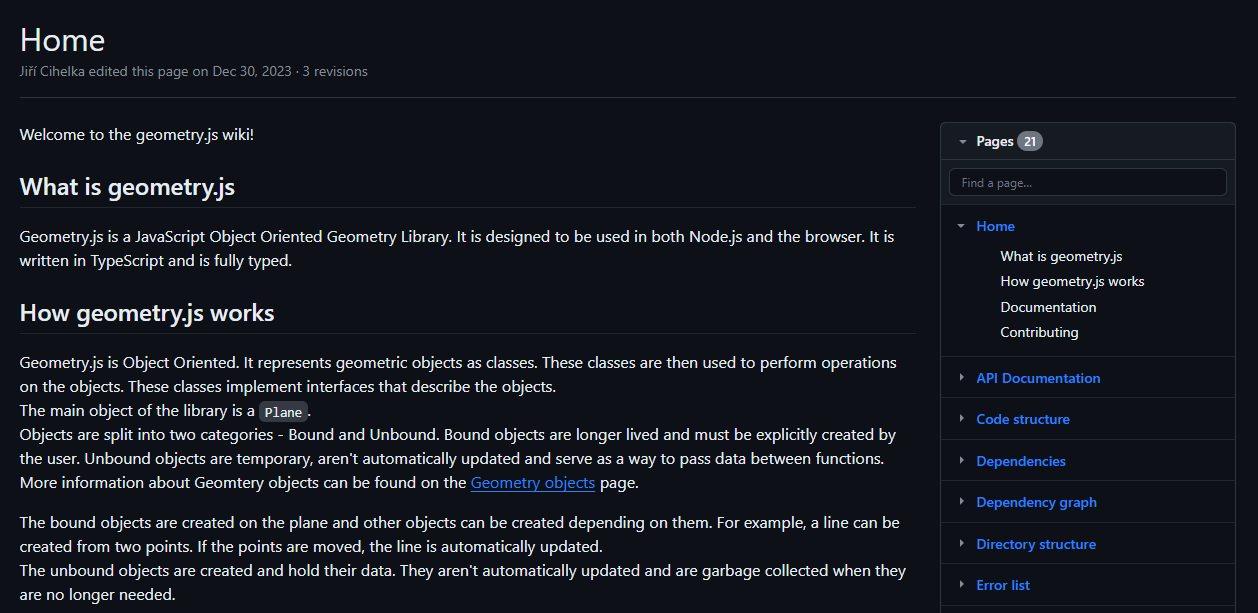
\includegraphics[height=0.6\textheight]{../resources/github-wiki-home.png}
        \caption{Ukázka domovské stránky GitHub Wiki.}
    \end{figure}
\end{frame}
